\documentclass[12pt, ]{scrartcl}
\usepackage[style=alphabetic]{biblatex}
\usepackage{graphicx}
\graphicspath{{./graphics}}
\addbibresource{bibliography.bib}
\usepackage{multicol}
\usepackage{setspace}
%opening
\title{Improvement of the Bayesian generalization model in order to handle negative examples and discontinuous hypotheses}

\begin{document}
\def\isblind{1}
\if\isblind0
    \author{Jason Cramer, Maximilian Dierschke, Nils Engleder}\fi
\if \isblind1
    \author{}\fi

\maketitle
\begin{abstract}
	abstract-text
\end{abstract}
\doublespacing
\begin{multicols}{2}
\section{Background}
The problem our project is focusing on is Shepard's ideal generalization problem. The generalization problem focuses on how humans build hypothesis spaces for a given consequence after observing stimuli.
In the paper "Generalization, similarity, and bayesian inference", they discuss how using a model of bayesian inference, we can predict the probability of given stimuli being included within the consequential region \cite{Tenenbaum}.
The model uses the equation $p(y \in C \mid x) = \sum\limits_{h:y\in h} p(h | x)$ where $h$ is a hypothesis from the hypothesis space ${\cal H}$ and $p(h | x)$ is the posterior probability of  the hypothesis after observing x.
We plan to extend this model to investigate how including negative examples within the x vector(x is the observed stimuli) affect how the model limits hypotheses. We also plan to explore how different distributions and models compare to the original model for generalization.
\section{Question}
To generalize the model by Tenenbaum et al, we want to find a way, how it can be improved, so that it can handle negative examples and discontinuous hypotheses.

\section{Negative examples in the baseline model}
The baseline model (Figure \ref{fig:baseline}), which was introduced by Tenenbaum et al. is by itself not capable of handling negative examples.

\begin{figure}[t]
	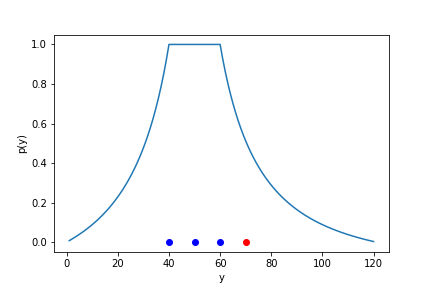
\includegraphics[width=4cm]{graphics/baseline.png}
	\centering
	\caption{Baseline model fitted on the positive examples [40, 50, 60] (red) does not incorporate the negative example [70] }
	\label{fig:baseline}
\end{figure}

A naive approach to incorporate negative examples, is to fit a model the same way it was fitted for the positive examples and then calculate the difference.
This then obviously needs to be 

\begin{figure}
	\centering
	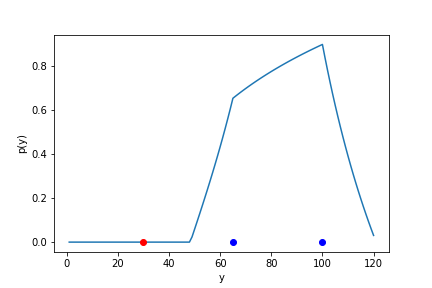
\includegraphics{graphics/addition_model}
	\caption{addition model fitted on the positive examples [40, 50, 60] (red) and negative exaample [70]}
\end{figure}
\noindent
In the graph we can see,
Evaluate how negative examples affect the predictions of the original model and use it as a baseline
(2) Evaluate the predictions made by the original model for multi cluster sample data
	
	
\section{Limiting positive regions using negative examples}
%(3) Evaluate how the model could be altered so that negative examples can be incorporated to limit cluster intervals assuming a continuous consequential region
A typical use case for negative samples under the assumption of a single positive region is limiting that region.
We would generally refer to the underlying thought process as one of elimination, which is why we shall call the corresponding model the elimination model.
Since our baseline model takes all possible hypotheses into consideration, the process of integrating counterexamples is relatively straightforward: We remove all those hypotheses from consideration which are contradicted by our negative examples.
To this end, we modify the likelihood calculation to

\section{Separating positive regions by negative examples}
%(4) Evaluate how the model could be altered so that negative examples can be incorporated to limit cluster intervals assuming a discontinuous consequential region


\section{Multiple Discontinuous Regions Model}
\begin{figure}
	\centering
	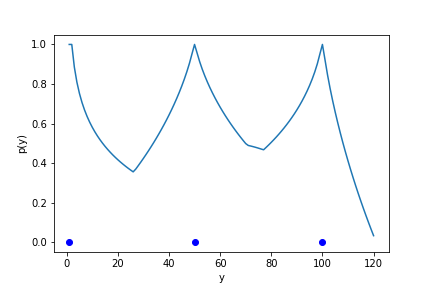
\includegraphics{graphics/mprm_model}
	\caption{Multiple discontinuous regions model fitted on examples [1, 100] with 2 disjoint regions.}
\end{figure}
(5) Evaluate how the model can be expanded to handle discontinuous regions without
negative examples
We want to initially solve the first three issues. Due to the added co

We start with a naive approach, where we will use the base model and fit one to positive and one to negative examples.

\centering

\nocite{*}
\printbibliography
\end{multicols}
\end{document}
